\documentclass[11pt,xcolor=dvipsnames,table]{beamer}
\usetheme{Szeged}
\usecolortheme{beaver}

\usepackage[utf8]{inputenc}
\usepackage[T1]{fontenc}
\usepackage[english]{babel}
\usepackage{amsmath}
\usepackage{amsfonts}
\usepackage{amssymb}
\usepackage{graphicx}
\usepackage{booktabs}
%\usepackage{tikz}
%\usetikzlibrary{calc,arrows,automata,shadows.blur,shapes,positioning,intersections}
\usepackage{hyperref}
\usepackage[absolute,overlay]{textpos}
%\usepackage[backend=biber, style=alphabetic, maxalphanames=1, sortlocale=en_US, natbib=true, url=false, doi=true, eprint=false, maxcitenames=1]{biblatex}
%\renewcommand*{\labelalphaothers}{}
\usepackage[algo2e]{algorithm2e}
\usepackage{caption}
\usepackage{subcaption}
\captionsetup{compatibility=false}
\usepackage{tabu}
\usepackage{multirow}
\usepackage{multicol}
%\addbibresource{References.bib}
%\bibliography{References}
%\renewcommand*{\bibfont}{\tiny} % resizes bibliography font size

\setbeamercolor{title}{fg=Brown,bg=Brown!20}
\setbeamercolor{frametitle}{fg=Brown,bg=Brown!20}
\setbeamercolor{section in head/foot}{bg=Brown}
\setbeamercolor{author in head/foot}{bg=Brown}
\setbeamercolor{date in head/foot}{fg=Brown}
\setbeamercolor*{item}{fg=Brown}


%\deftranslation[to=portuguese]{Theorem}{Teorema}
%\deftranslation[to=portuguese]{Proof}{Prova}

\defbeamertemplate*{footline}{shadow theme}
{%
	\leavevmode%
	\hbox{\begin{beamercolorbox}[wd=.5\paperwidth,ht=2.5ex,dp=1.125ex,leftskip=.3cm plus1fil,rightskip=.3cm]{author in head/foot}%
			\usebeamerfont{author in head/foot}\insertframenumber\,/\,\inserttotalframenumber\hfill\insertshortauthor
		\end{beamercolorbox}%
		\begin{beamercolorbox}[wd=.5\paperwidth,ht=2.5ex,dp=1.125ex,leftskip=.3cm,rightskip=.3cm plus1fil]{title in head/foot}%
			\usebeamerfont{title in head/foot}\insertshorttitle%
		\end{beamercolorbox}}%
		\vskip0pt%
	}

\AtBeginSection[]
{
	\begin{frame}{Index}
		\tableofcontents[currentsection, currentsubsection]
	\end{frame}
}

\AtBeginSubsection[]
{
	\begin{frame}{Index}
		\tableofcontents[currentsection, currentsubsection]
	\end{frame}
}

\author[Ramon Costi Fernandes]{\textbf{Priscila Giovanella Vivian} \\ \vspace{20pt} {\scriptsize \textbf{Advisor: Prof. Ph.D. César Augusto Missio Marcon \\ Co-Advisor: Prof. Ph.D. Martha Johanna Sepúlveda Flórez}}}
\title{A Security Aware Routing Approach for Networks-on-Chip}
%\subtitle{}
%\logo{
\includegraphics[scale=0.35]{logo-pucrs.jpg}\hspace{1.05\linewidth}
\includegraphics[scale=0.35]{logo-facin.jpg}}
\institute[]{Pontifical Catholic University of Rio Grande do Sul\\Faculty of Informatics\\Computer Science Graduate Program}
\date{July 20, 2016}
%\subject{}
%\setbeamercovered{transparent}
%\setbeamertemplate{navigation symbols}{}

\begin{document}

	%%%%%%%%%%%%%%%%%%%%%%%%%%%%%%%%%%%%%%%%%%
	%%% TITLE PAGE %%%%%%%%%%%%%%%%%%%%%%%%%%%
	%%%%%%%%%%%%%%%%%%%%%%%%%%%%%%%%%%%%%%%%%%
	{
		\setbeamertemplate{headline}{}
		\setbeamertemplate{footline}{}
		\begin{frame}
			\titlepage
		\end{frame}
	}
	\addtocounter{framenumber}{-1} %desconta o primeiro slide da numeracao
	
	%%%%%%%%%%%%%%%%%%%%%%%%%%%%%%%%%%%%%%%%%%
	%%% INDEX %%%%%%%%%%%%%%%%%%%%%%%%%%%%%%%%
	%%%%%%%%%%%%%%%%%%%%%%%%%%%%%%%%%%%%%%%%%%
	\begin{frame}{Index}
		\tableofcontents
	\end{frame}
	
	%%%%%%%%%%%%%%%%%%%%%%%%%%%%%%%%%%%%%%%%%%
	%%% INTRODUCTION %%%%%%%%%%%%%%%%%%%%%%%%%
	%%%%%%%%%%%%%%%%%%%%%%%%%%%%%%%%%%%%%%%%%%
	\section{Introduction}\label{sec:intro}
\begin{frame}[allowframebreaks]{Introduction}
	\begin{itemize}
		\setlength{\itemsep}{0.5em}
		\item<1-> The Network-on-Chip (NoC) has been widely adopted as a paradigm capable of providing a reliable and scalable interconnection in MPSoCs \cite{sgroi_addressing_2001}, \cite{ye_packetization_2004}
		
		\item<1-> The concern for data protection appears as a design requirement of MPSoCs
		
		\item<1-> Protection usually occurs at either:
			\begin{itemize}
				\setlength{\itemsep}{0.5em}
				\item<1-> \emph{Application Level}, e.g.,\ using data encryption or source authentication; or
				\item<1-> \emph{Communication Level}, e.g.,\ detecting abnormal communication behavior in the system.
			\end{itemize}
		
		\item<1-> NoCs have been shown to aid in the overall MPSoC protection \cite{diguet_noc-centric_2007}, \cite{sepulveda_noc-based_2015}, \cite{grammatikakis_security_2014}, by implementing security services at communication level
	\end{itemize}
\end{frame}

%%%%%%%%%%%%%%%%%%%%%%%%%%%%%%%%%%%%%%%%%%
%%% OBJECTIVES %%%%%%%%%%%%%%%%%%%%%%%%%%%
%%%%%%%%%%%%%%%%%%%%%%%%%%%%%%%%%%%%%%%%%%
\subsection{Objectives}\label{sec:objectives}
\begin{frame}{Objectives}
	\begin{itemize}
		\setlength{\itemsep}{1em}
		\item<1-> The definition of a routing model that is capable of considering system security requirements to define safe routing paths
		
		\item<1-> The creation of an abstract model that enables the implementation and the verification of the routing technique
		
		\item<1-> The validation and evaluation of the routing algorithm for different security configurations
		
		\item<1-> The adaptation of an existing NoC simulation platform to employ this new routing model for behavior evaluation
	\end{itemize}
\end{frame}
	
	%%%%%%%%%%%%%%%%%%%%%%%%%%%%%%%%%%%%%%%%%%
	%%% PROJECT PROPOSAL %%%%%%%%%%%%%%%%%%%%%
	%%%%%%%%%%%%%%%%%%%%%%%%%%%%%%%%%%%%%%%%%%
	\section{Research}\label{sec:proposal}
\begin{frame}{Research}
	\begin{itemize}
		\setlength{\itemsep}{1em}
		\item<1-> This work is based on two premises:
		
		\begin{enumerate}[(i)]
			\setlength{\itemsep}{1em}
			\item<1-> that sensitive applications communicate over the NoC in MPSoCs, and are therefore vulnerable to interference by malicious applications; and
			
			\item<1-> that protection from software attacks is achieved by communication level protection; e.g., by defining safe communication paths for sensitive applications
		\end{enumerate}
		
		\item<1-> Therefore, a routing algorithm that is capable of defining safe routing paths for sensitive applications should enhance the overall system protection
	\end{itemize}
\end{frame}

%%%%%%%%%%%%%%%%%%%%%%%%%%%%%%%%%%%%%%%%%%
%%% THREAT MODEL %%%%%%%%%%%%%%%%%%%%%%%%%
%%%%%%%%%%%%%%%%%%%%%%%%%%%%%%%%%%%%%%%%%%
\subsection{Threat Model}
\begin{frame}{Threat Model}
	\begin{center}
		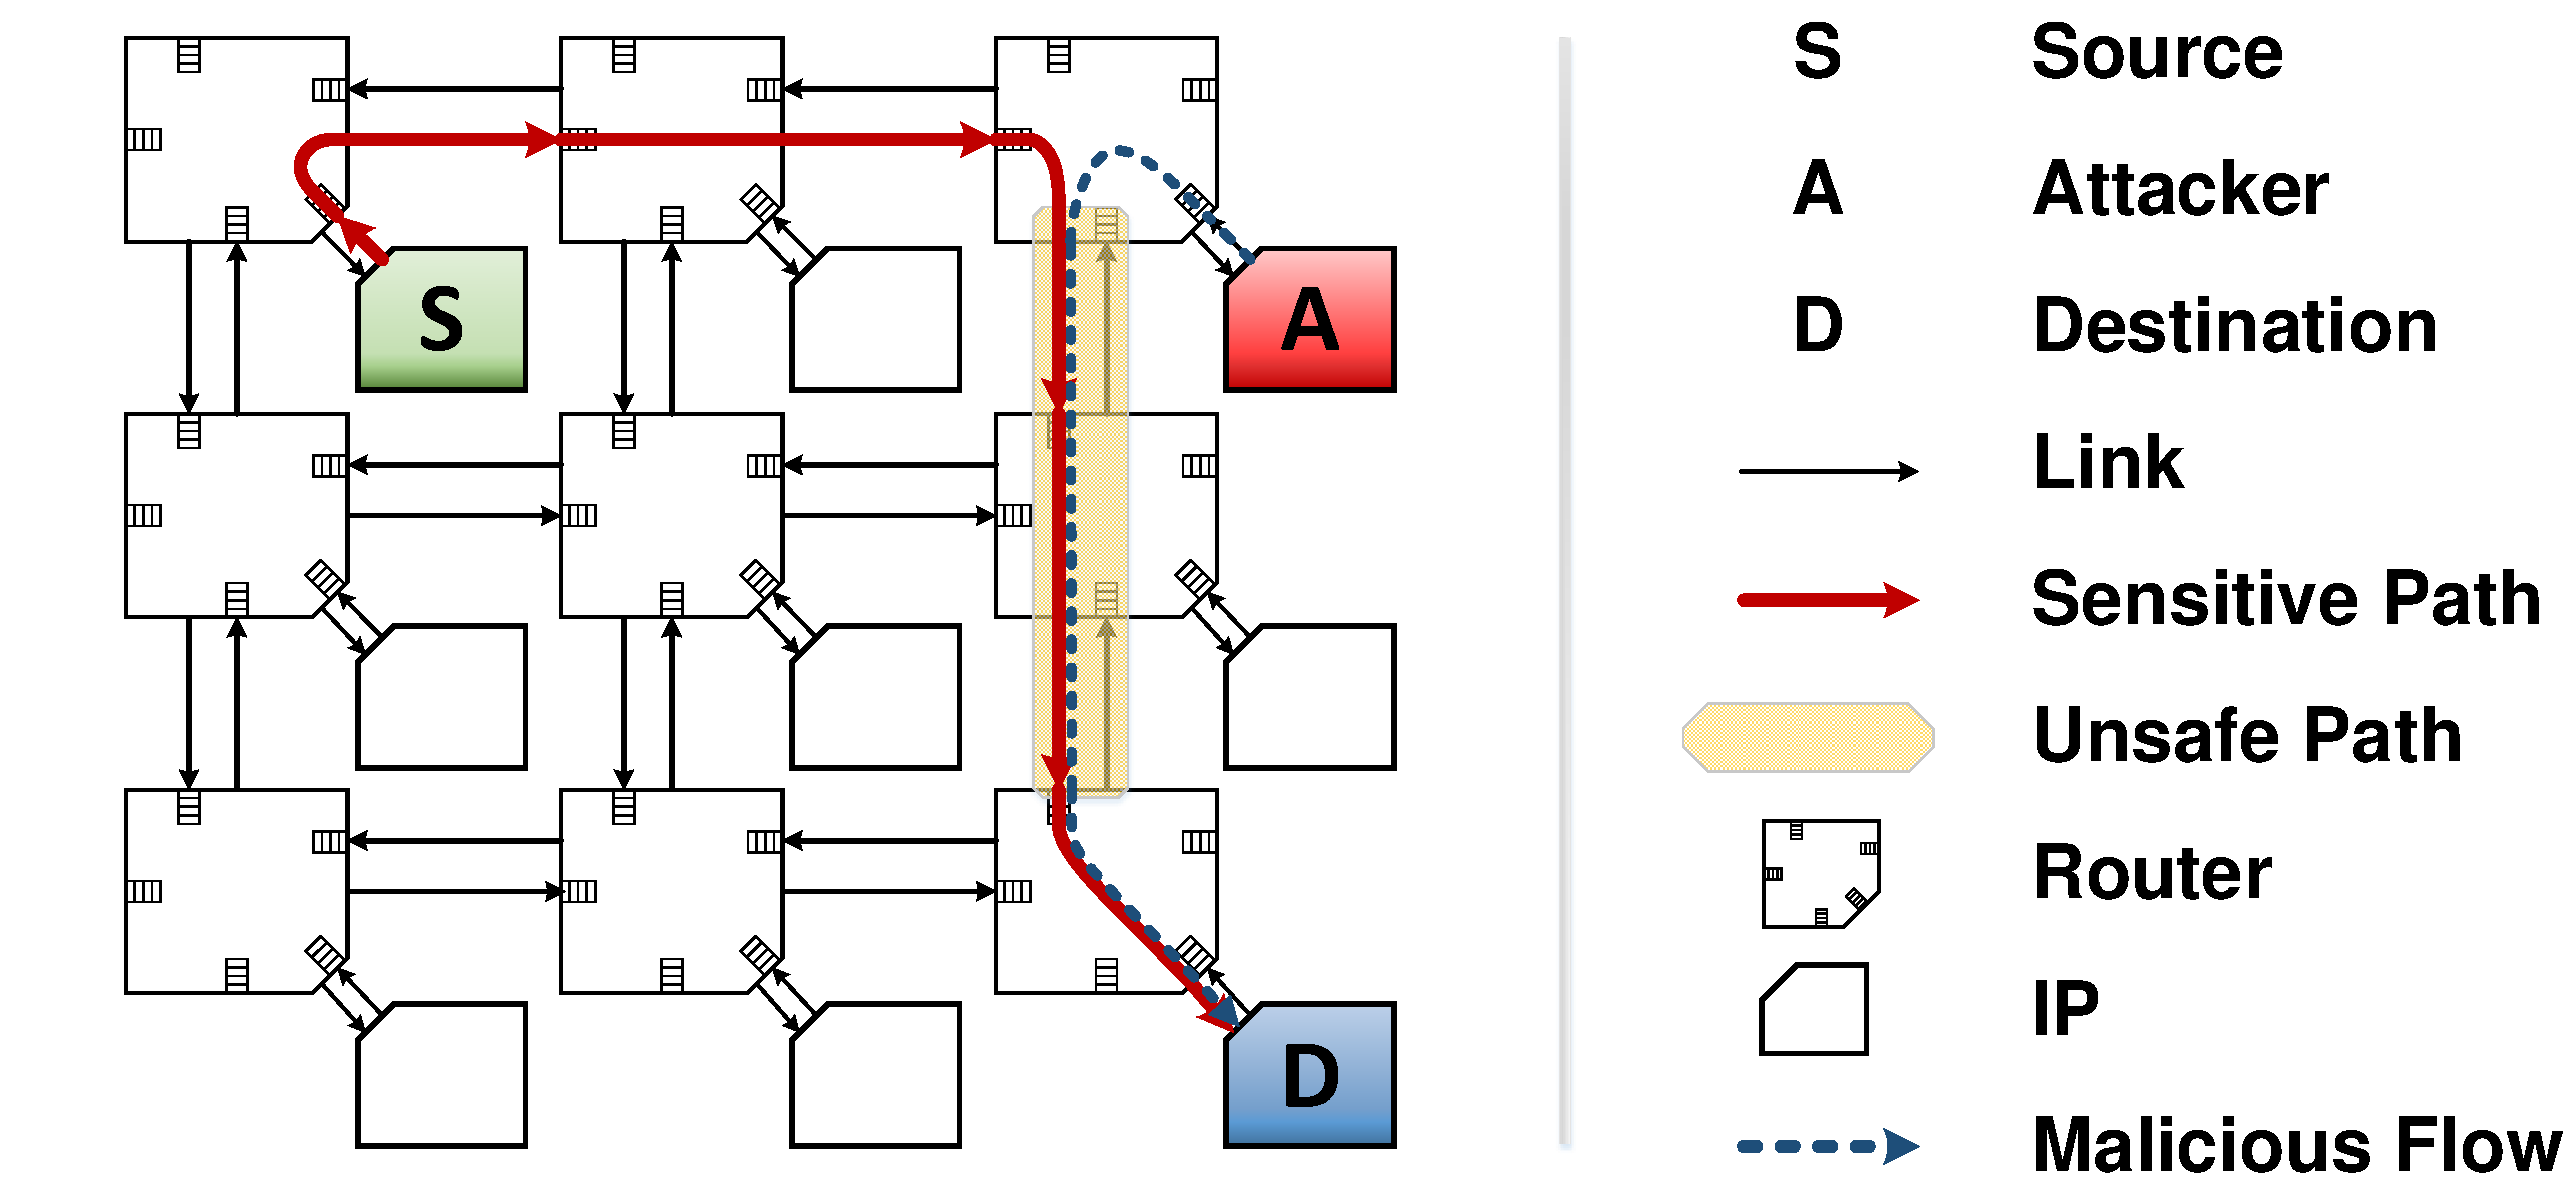
\includegraphics[width=0.75\linewidth]{images/threat_model/timing-attack.pdf}
	\end{center}
	\begin{itemize}
		\item<only@1> The NoC is considered secure, meaning that an attacker cannot tamper its resources
		
		\item<only@1> An attacker, aware of the sensitive path, can disrupt communication between a source and a destination
		
		\item<only@1> We consider that an attacker can either generate a \emph{DoS} or \emph{Timing Attack} on the sensitive path
	\end{itemize}
\end{frame}

%%%%%%%%%%%%%%%%%%%%%%%%%%%%%%%%%%%%%%%%%%
%%% SECURITY AWARE ROUTING %%%%%%%%%%%%%%%
%%%%%%%%%%%%%%%%%%%%%%%%%%%%%%%%%%%%%%%%%%
\subsection{Security Aware Routing}
\begin{frame}{Security Zones}
	\begin{center}
		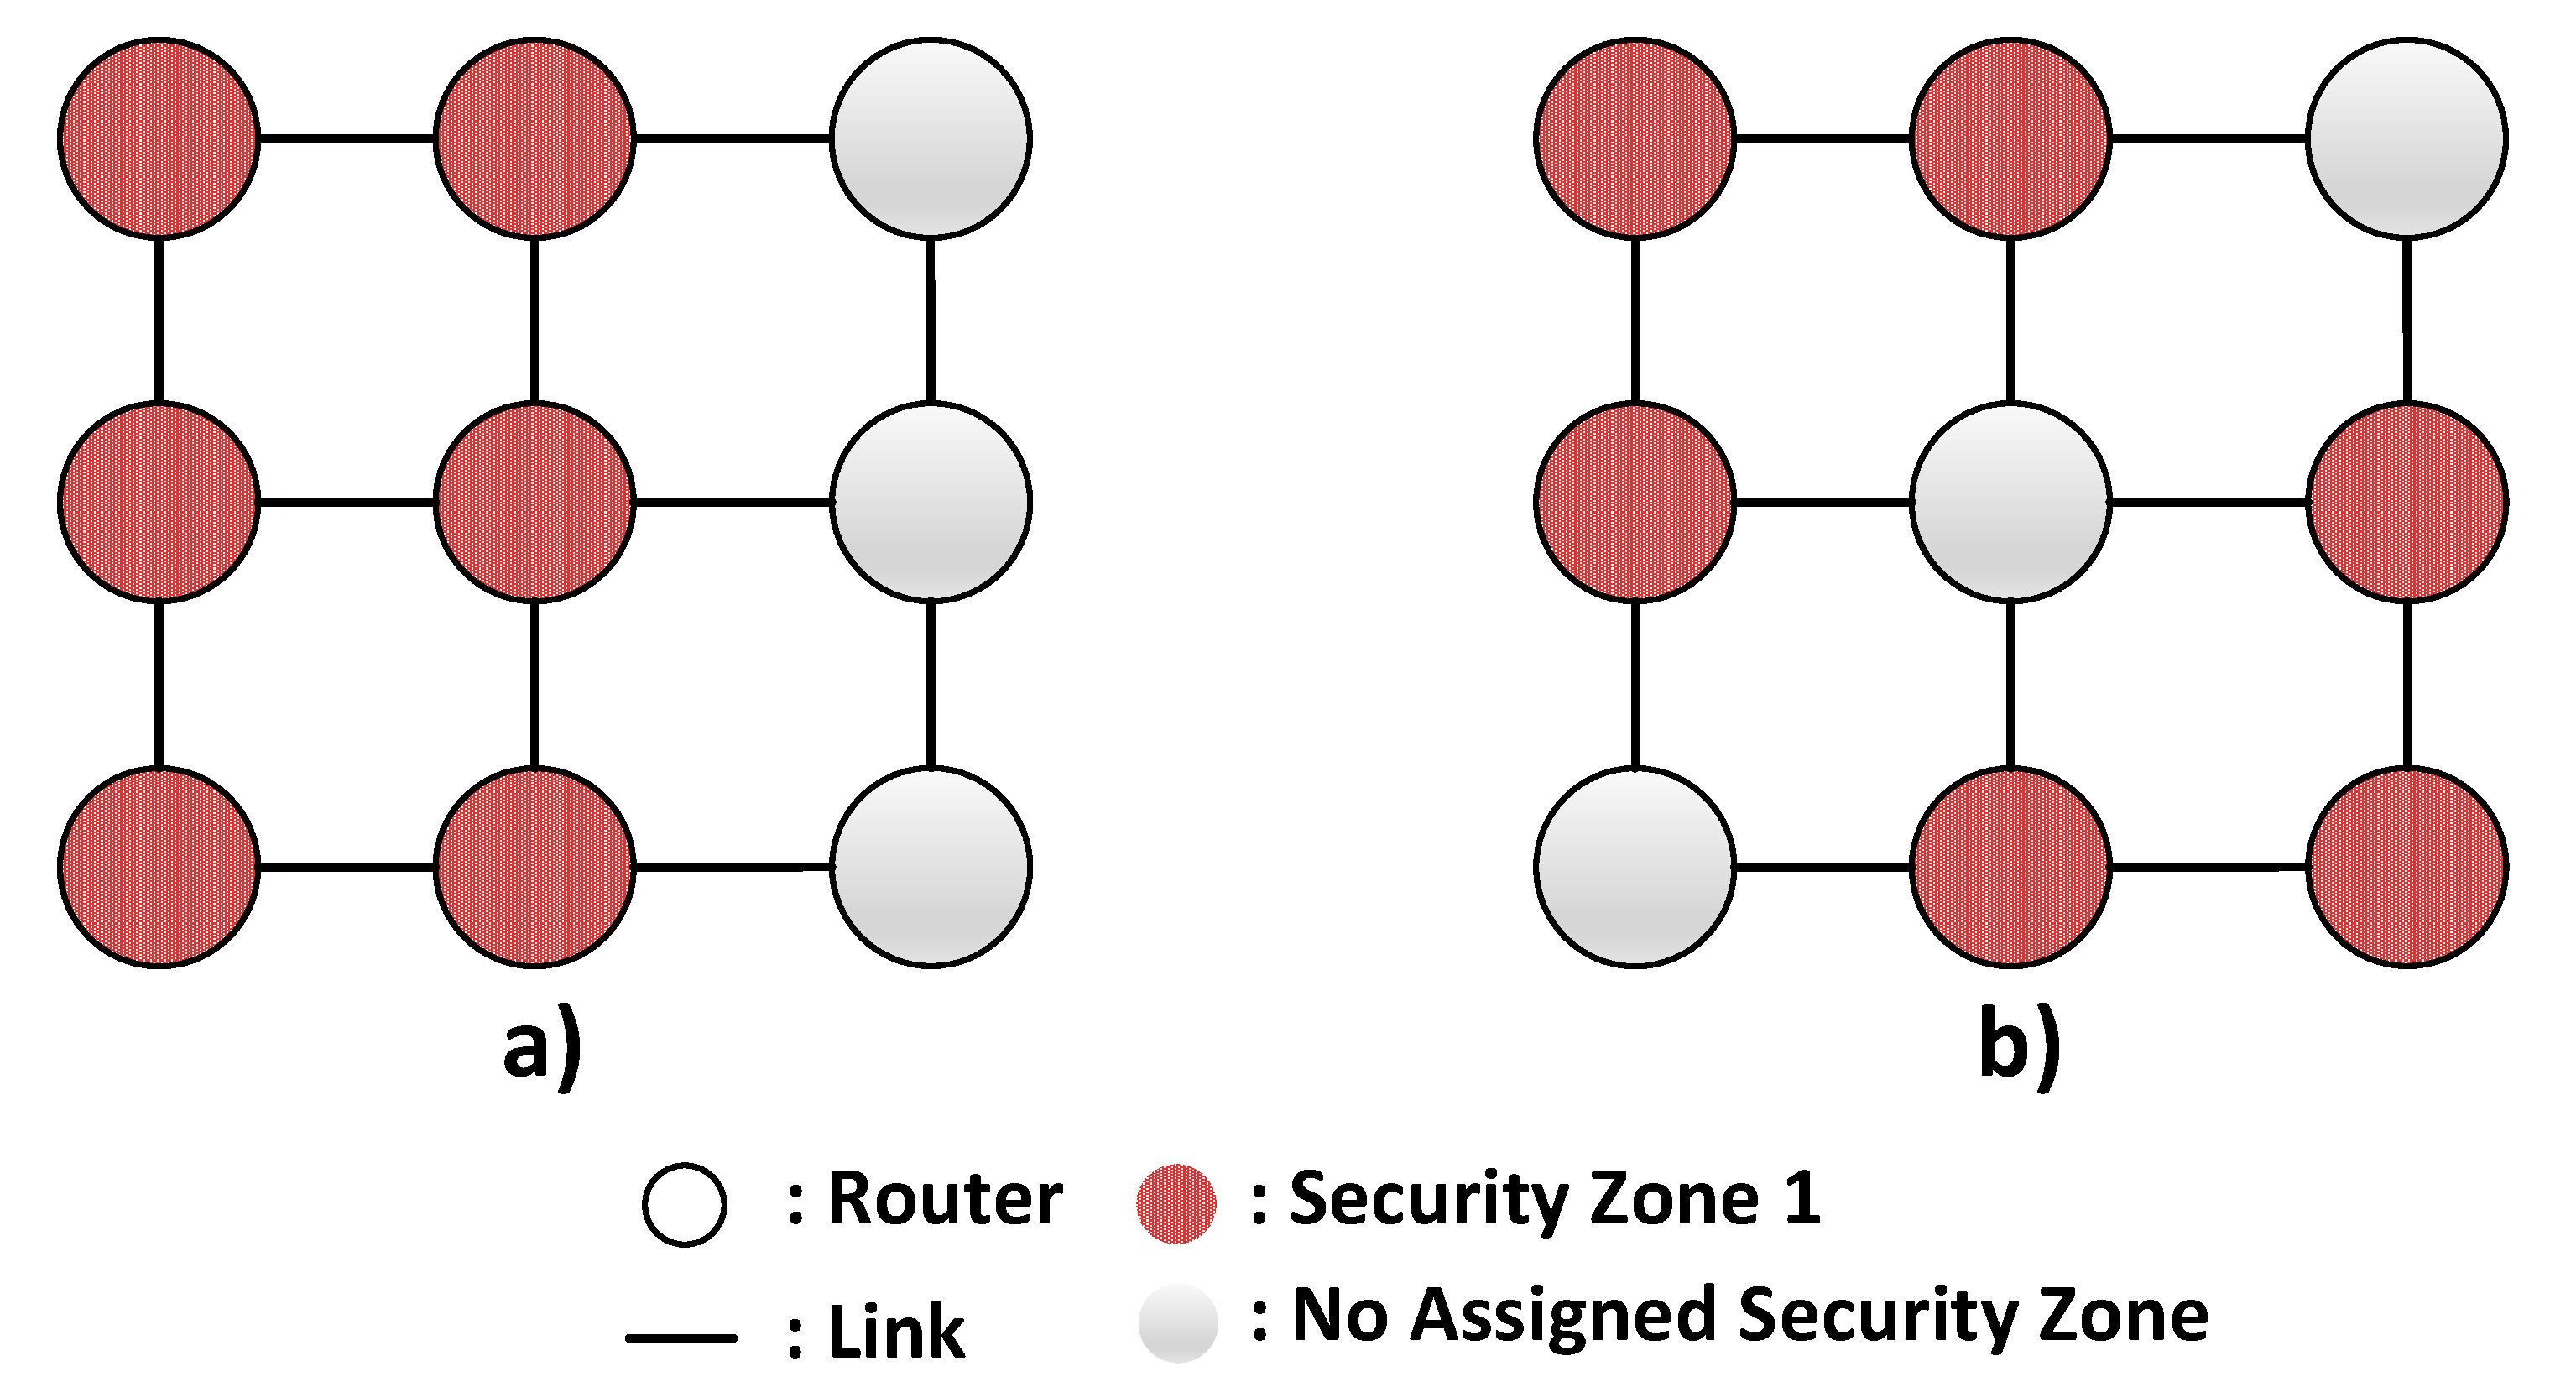
\includegraphics[width=0.60\linewidth]{images/secure_routing/security-zones-shapes.pdf}
	\end{center}
	\begin{itemize}
		\item<only@1> A security zone is a physical space (continuous or disrupted) that wraps IPs that execute critical applications
		
		\item<only@1> The task mapping of critical applications defines the shape of the security zone
		
		\item<only@1> Certain IP blocks might not be assigned to any security zone, e.g., idle resources or shared memories
	\end{itemize}
\end{frame}
\begin{frame}[t]{Communication in Security Zones}
	\begin{onlyenv}<1-3>
		\begin{center}
			\includegraphics<1>[width=0.85\linewidth]{images/secure_routing/security-zones-fiz.pdf}
			\includegraphics<2>[width=0.85\linewidth]{images/secure_routing/security-zones-piz.pdf}
			\includegraphics<3>[width=0.85\linewidth]{images/secure_routing/security-zones-iz.pdf}
		\end{center}
	\end{onlyenv}
	\begin{itemize}
		\item<only@1> \textit{\textbf{Full intra-zone communication (FIZ)}}: \emph{S} and \emph{D} are in the same $SZ$. The sensitive path is \textbf{completely} inside the $SZ$, e.g., the path from \emph{IP1} to \emph{IP2}
		
		\item<only@2> \textbf{\textit{Partial intra-zone communication (PIZ)}}: \emph{S} and \emph{D} are in the same $SZ$. However, the sensitive path is \textbf{partially} inside the $SZ$. , e.g., the path from \emph{IP3} to \emph{IP4}
		
		\item<only@3> \textbf{\textit{Inter-zone communication (IZ)}}: \emph{S} and \emph{D} are in different $SZ$, e.g., the path from \emph{IP5} to \emph{IP6}
	\end{itemize}
\end{frame}

\begin{frame}[t]{Segment-based Routing (SBR) - Deadlock Prevention}
	\begin{center}
		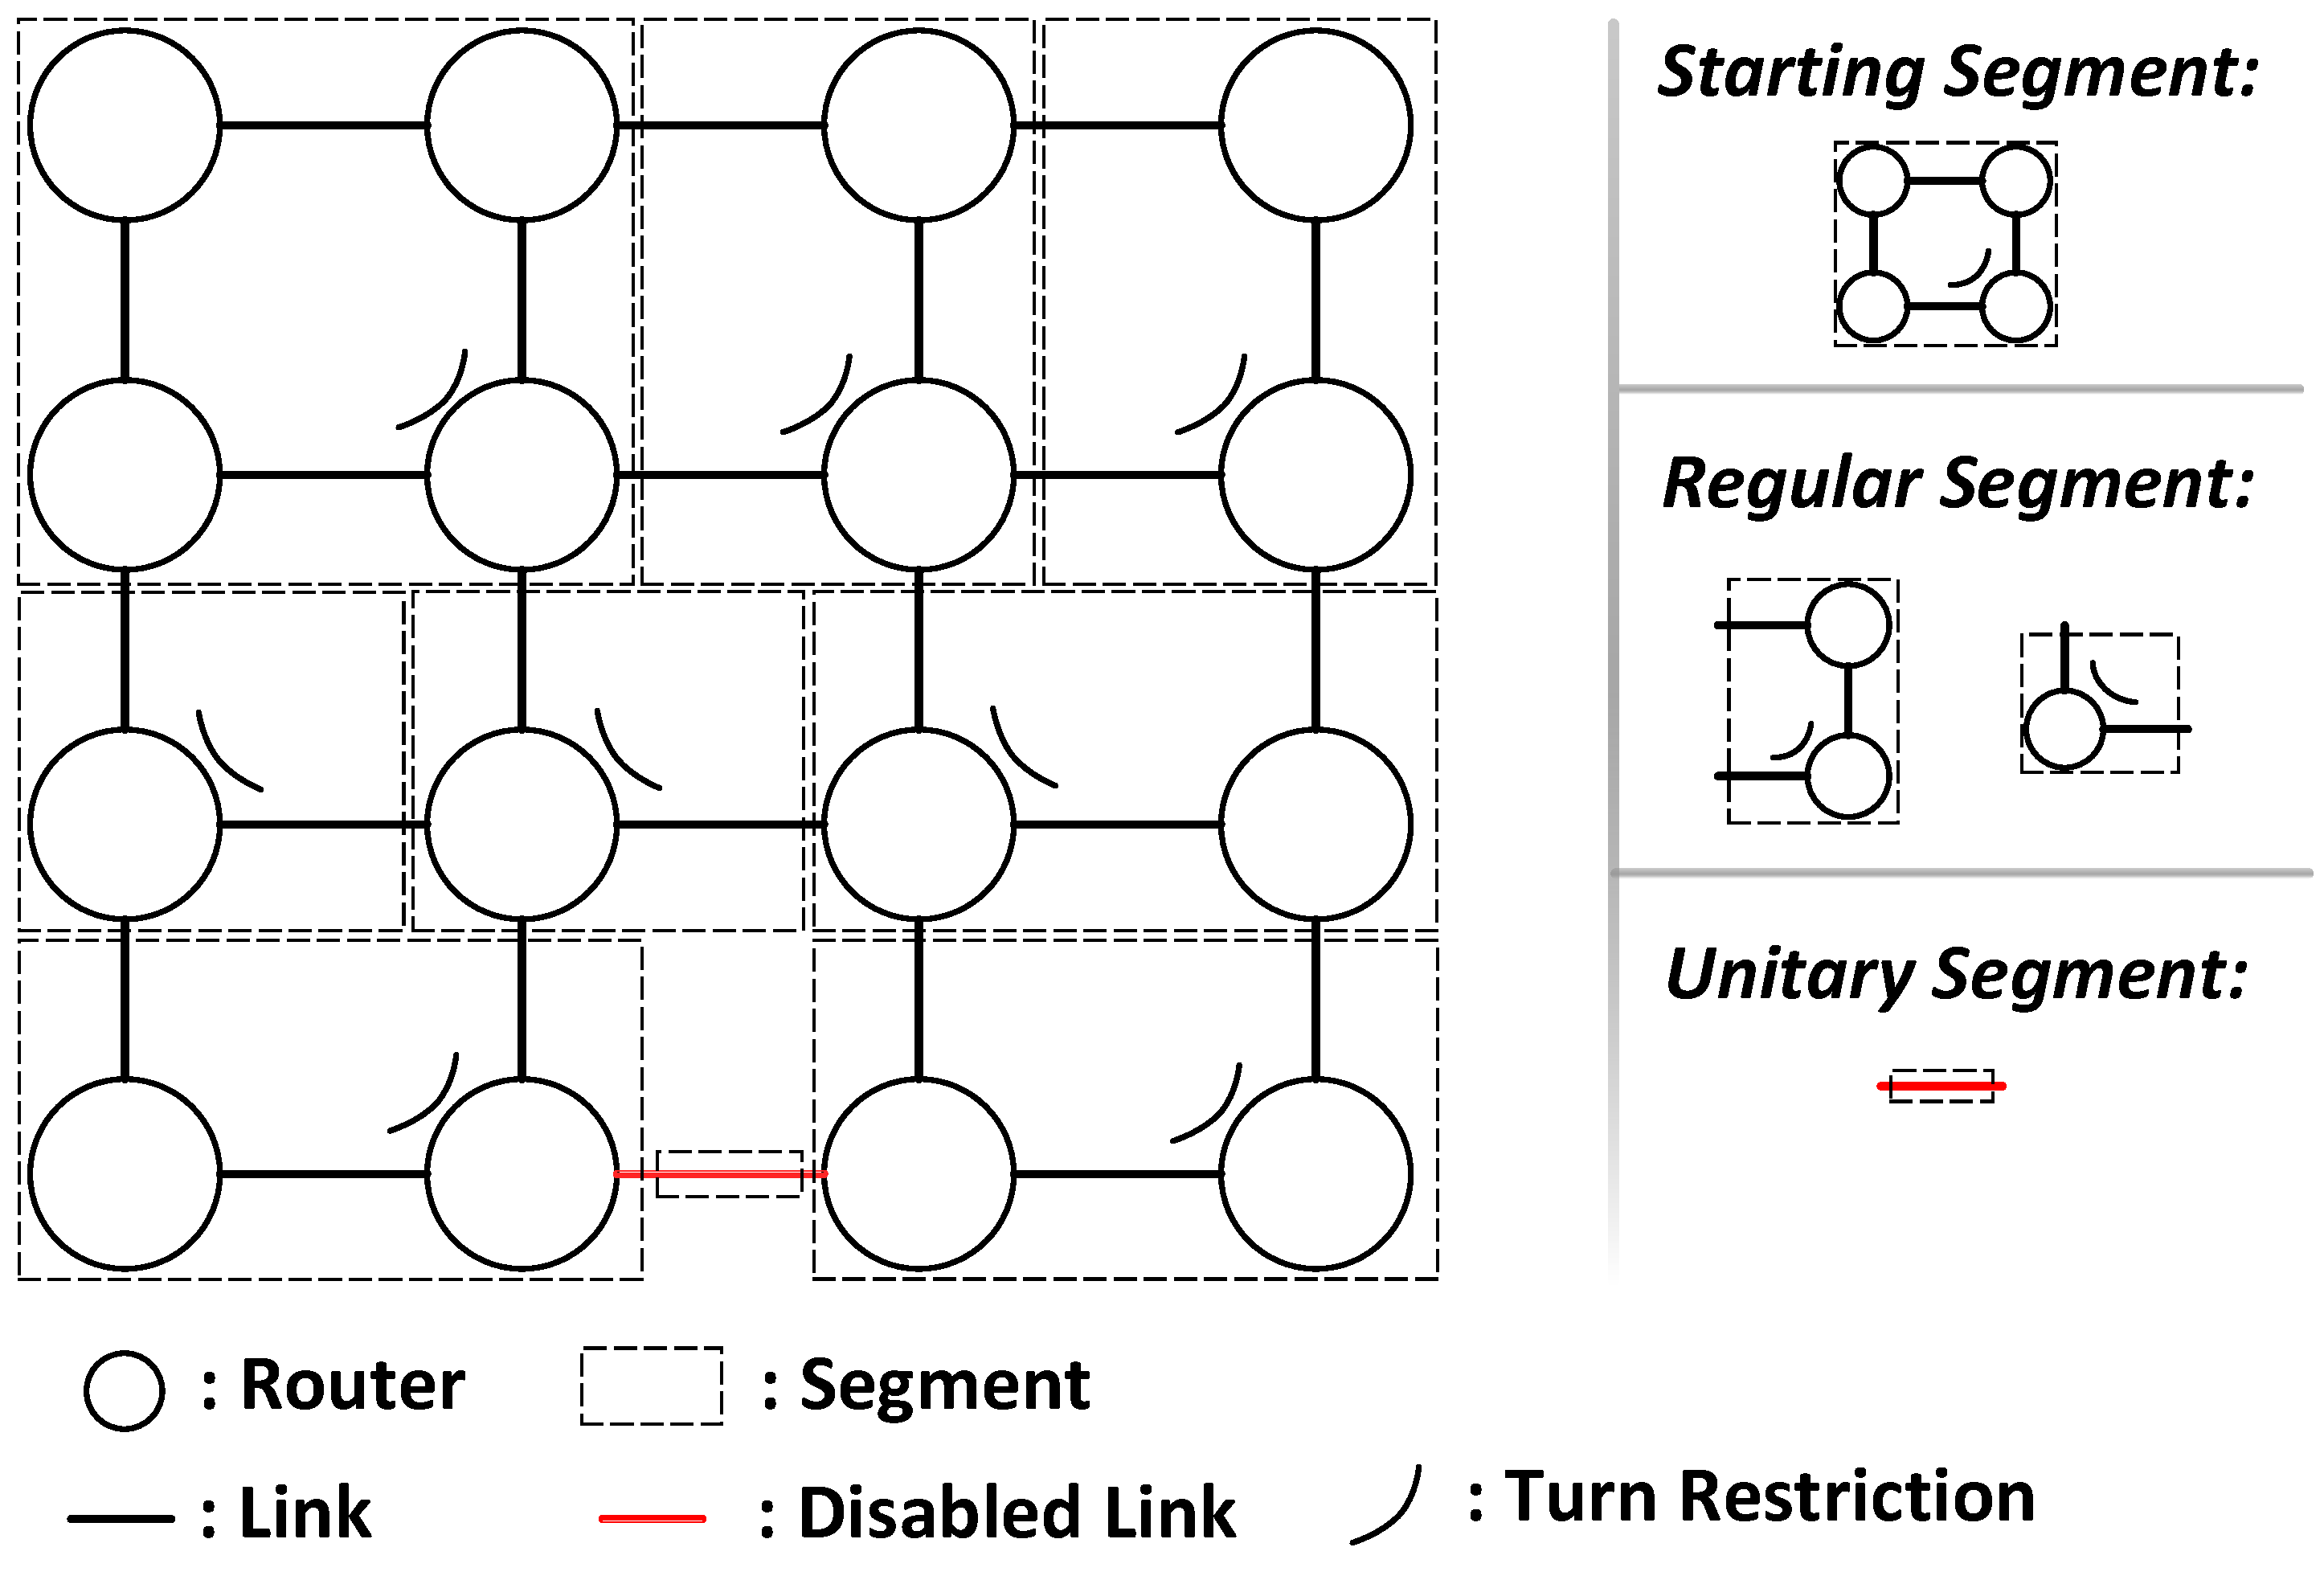
\includegraphics[width=0.65\linewidth]{images/secure_routing/sbr.pdf}
	\end{center}
	\begin{itemize}
		\item<only@+> Logically partitions the NoC into segments
		
		\item<only@+> Each segment contains a localized bidirectional turn restriction
		
		\item<only@+> Guarantees global deadlock freedom and reachability (as long as the NoC is connected)
	\end{itemize}
\end{frame}

\begin{frame}[t]{SBR-Security Zone Awareness (SBR-SZA)}
	\begin{onlyenv}<1-2>
		\begin{center}
			\includegraphics<1>[width=0.85\linewidth]{images/secure_routing/sbr-configs.pdf}
			\includegraphics<2>[width=0.75\linewidth]{images/secure_routing/sbr-sza.pdf}
		\end{center}
	\end{onlyenv}
	\begin{itemize}
		\item<only@1> Traditional SBR might place turn restrictions that causes \textbf{\textit{PIZ}} routing
		\item<only@2> SBR-SZA aims to create segments that tailor to security zone shapes
	\end{itemize}
\end{frame}

\begin{frame}{Region-based Routing (RBR) - Routing Algorithm}
	\begin{itemize}
		\setlength{\itemsep}{1em}
		\item<1-> Populates the routing tables of NoC routers, considering the turn restrictions of SBR
		
		\item<1-> Groups routing entries to greatly reduce table size (interval routing and port/destination sets)
		
		\item<1-> There are three steps in RBR computation:
		\begin{itemize}[i]
			\setlength{\itemsep}{0.5em}
			\item<1-> \textit{Routing Computation}: computes all source and destination pairs
			
			\item<1-> \textit{Region Computation}: joins entries based on input and output ports
			
			\item<1-> \textit{Region Merge}: merges overlapping regions to reduce routing entries
		\end{itemize}
	\end{itemize}
\end{frame}

%%%%%%%%%%%%%%%%%%%%%%%%%%%%%%%%%%%%%%%%%%
%%% MODELING %%%%%%%%%%%%%%%%%%%%%%%%%%%%%
%%%%%%%%%%%%%%%%%%%%%%%%%%%%%%%%%%%%%%%%%%
\subsection{Modeling}
\begin{frame}[t]{Modeling}
	\begin{center}
		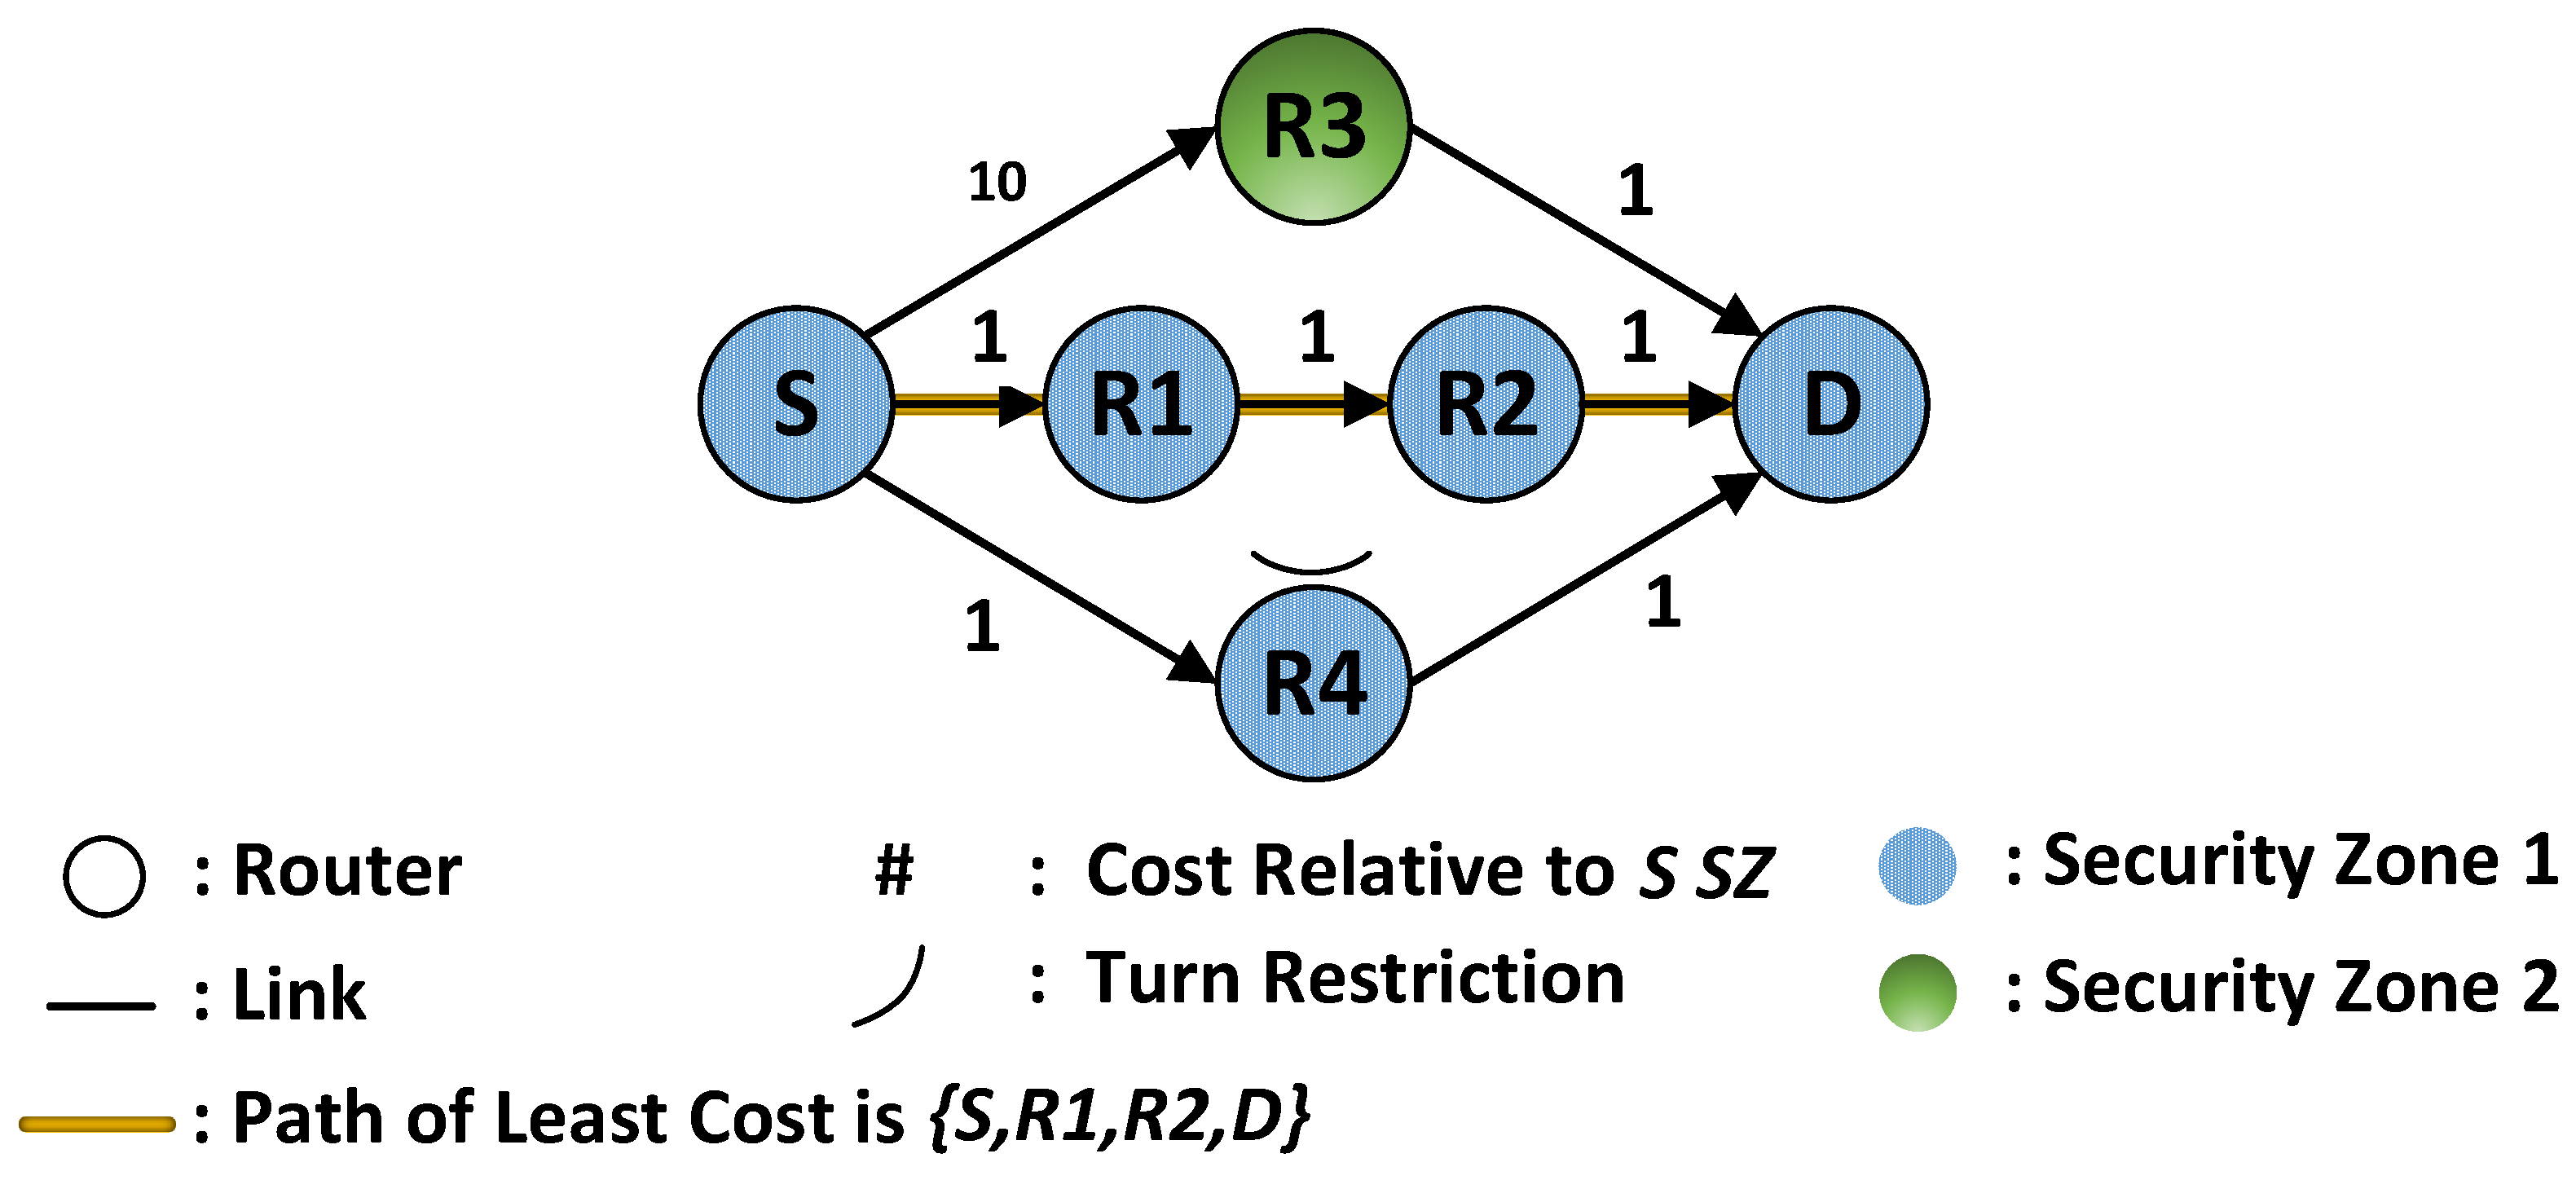
\includegraphics[width=0.75\linewidth]{images/secure_routing/rbr-path-finding.pdf}
	\end{center}
	\begin{itemize}
		\item<only@1> The NoC is modeled as a graph, with IP/Routers as vertices and links as edges
		
		\item<only@2> Each vertex belongs to a security zone, and each edge has a positive weight that is set according to the path-finding iteration
		
		\item<only@3> Edge weight can represent the cost to employ encryption to a sensitive packet
	\end{itemize}
\end{frame}

	
	%%%%%%%%%%%%%%%%%%%%%%%%%%%%%%%%%%%%%%%%%%
	%%% EVALUATION AND RESULTS %%%%%%%%%%%%%%%
	%%%%%%%%%%%%%%%%%%%%%%%%%%%%%%%%%%%%%%%%%%
	\section{Evaluation}\label{sec:evaluation}
\begin{frame}[t]{NoC Configuration Tool}
	\begin{center}
		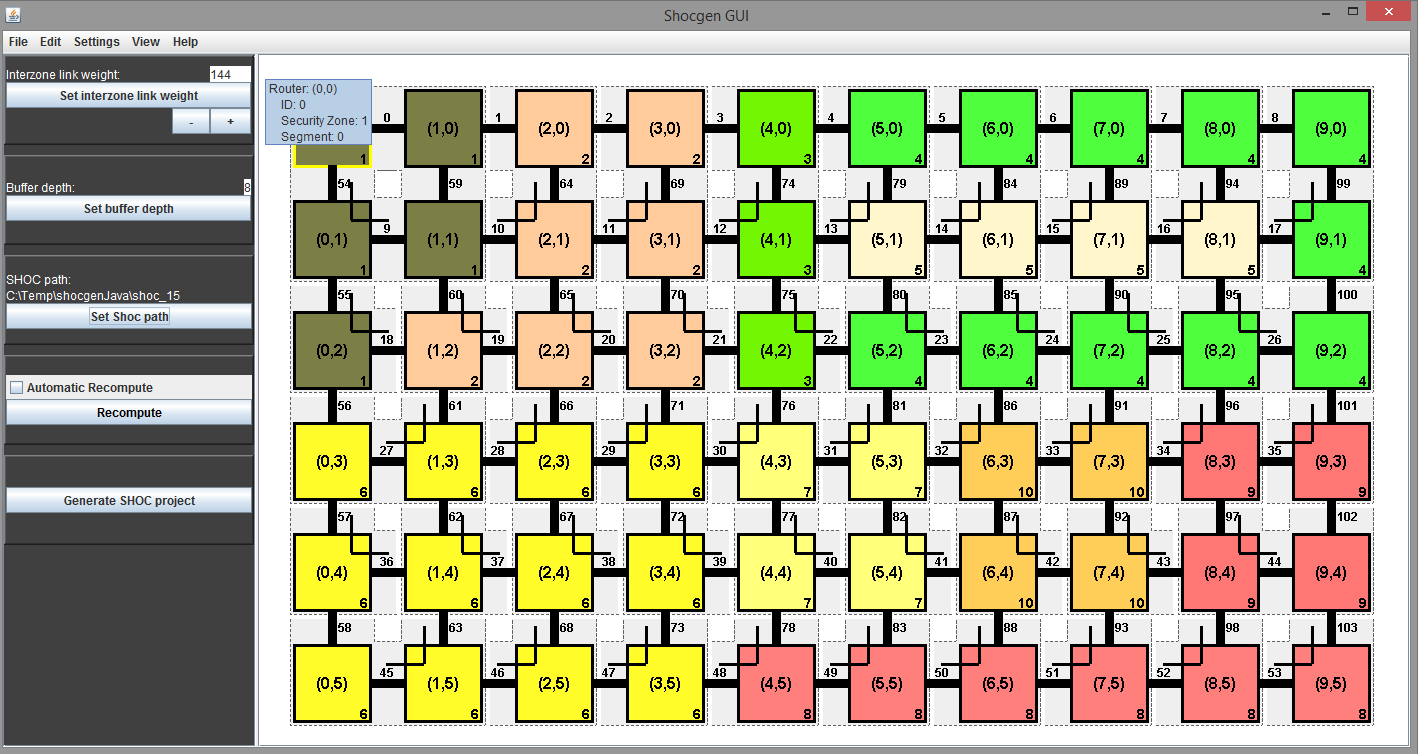
\includegraphics[width=0.75\linewidth]{images/evaluation/shocgentool.png}
	\end{center}
	\begin{itemize}
		\item<only@1> Graphical configuration tool to generate and compute scenarios at \textit{design time}
		
		\item<only@2> Implements SBR and RBR algorithms to populate routing entries
		
		\item<only@3> Performs routing entries, \textbf{\textit{FIZ/PIZ}} routing paths, and latency evaluations
		
		\item<only@4> Outputs the generated configuration to a SystemC simulation platform
	\end{itemize}
\end{frame}

%%%%%%%%%%%%%%%%%%%%%%%%%%%%%%%%%%%%%%%%%%
%%% EVALUATION CRITERIA %%%%%%%%%%%%%%%%%%
%%%%%%%%%%%%%%%%%%%%%%%%%%%%%%%%%%%%%%%%%%
\subsection{Evaluation Criteria}
\begin{frame}[t]{Evaluation Criteria}
	\begin{center}
		\resizebox{1.0\linewidth}{!}
		{
			\begin{tabular}{c|c|c|c|c}
				\toprule[2pt]
				Scenario & NoC Dimension (Columns $X$ Rows) & SBR Seeds & Segmentation Modes & Configurations per Scenario\\
				\midrule[1.5pt]
				NASA NAS & 13x13         & 169       & \emph{SBR} / \emph{SBR-SZA} &338 \\
				\hline
				Synth 1  & 6x4           & 24        & \emph{SBR} / \emph{SBR-SZA} &48  \\
				\hline
				Synth 2  & 10x6          & 60        & \emph{SBR} / \emph{SBR-SZA} &120 \\
				\midrule[1.5pt]
				\multicolumn{4}{r|}{Total:}                                        &506 \\
				\bottomrule[2pt]
			\end{tabular}
		}
	\end{center}
	
	\begin{itemize}
		\setlength{\itemsep}{1em}
		\item<only@1> Three scenarios evaluated: 2 synthetic and 1 based on a real application communication dependency trace
		
		\item<only@1> Evaluation consists of four preliminary steps
		\begin{itemize}[i]
			\setlength{\itemsep}{0.5em}
			\item<only@1> Seed for segment computation
			
			\item<only@1> SBR computation
			
			\item<only@1> RBR computation
			
			\item<only@1> Evaluation of obtained configuration
		\end{itemize}
		
		\setlength{\itemsep}{1em}
		\item<only@2> Three evaluations were performed:
		\begin{itemize}[i]
			\setlength{\itemsep}{0.5em}
			\item<only@2> Routing table scalability
			
			\item<only@2> \textbf{\textit{FIZ/PIZ}} occurrences
			
			\item<only@2> Latency estimation
		\end{itemize}
	\end{itemize}
\end{frame}

%%%%%%%%%%%%%%%%%%%%%%%%%%%%%%%%%%%%%%%%%%
%%% PRELIMINARY RESULTS %%%%%%%%%%%%%%%%%%
%%%%%%%%%%%%%%%%%%%%%%%%%%%%%%%%%%%%%%%%%%
\subsection{Preliminary Results}
\begin{frame}{Routing Table Scalability - Average Routing Tables Size}
	\begin{center}
		\begin{figure}
			\begin{subfigure}{0.49\linewidth}
				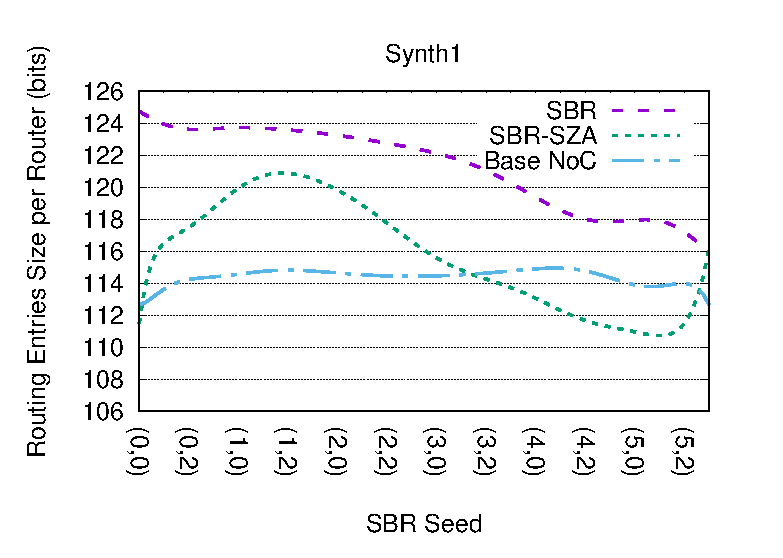
\includegraphics[width=1.0\linewidth]{charts/synth1/synth1-routing-tables-bits-bezier.eps}
			\end{subfigure}
			\begin{subfigure}{0.49\linewidth}
				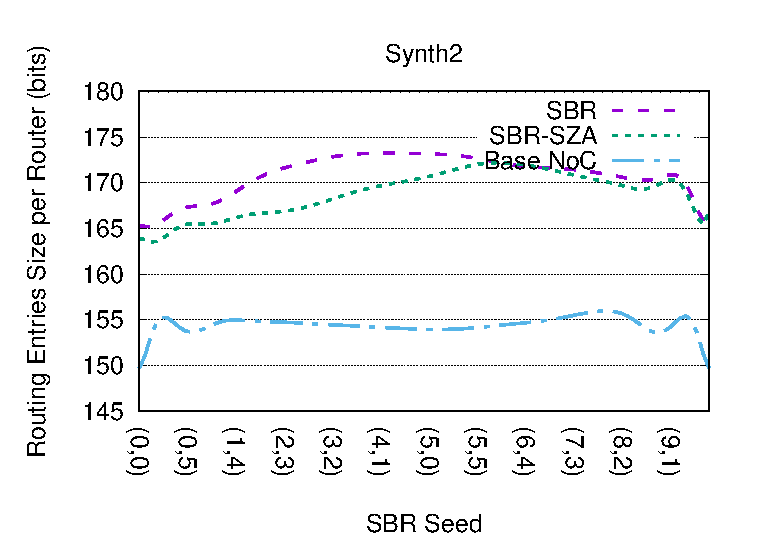
\includegraphics[width=1.0\linewidth]{charts/synth2/synth2-routing-tables-bits-bezier.eps}
			\end{subfigure}
			\begin{subfigure}{0.49\linewidth}
				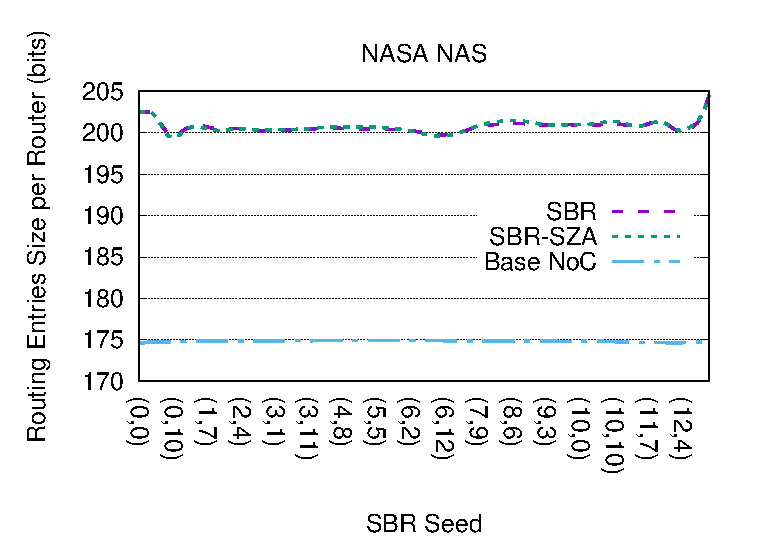
\includegraphics[width=1.0\linewidth]{charts/nasa/nasa-routing-tables-bits-bezier.eps}
			\end{subfigure}
		\end{figure}
	\end{center}
\end{frame}

\begin{frame}{Routing Table Scalability - Optimal Configuration Heatmap}
	\begin{center}
		\begin{figure}
			\begin{subfigure}{0.45\linewidth}
				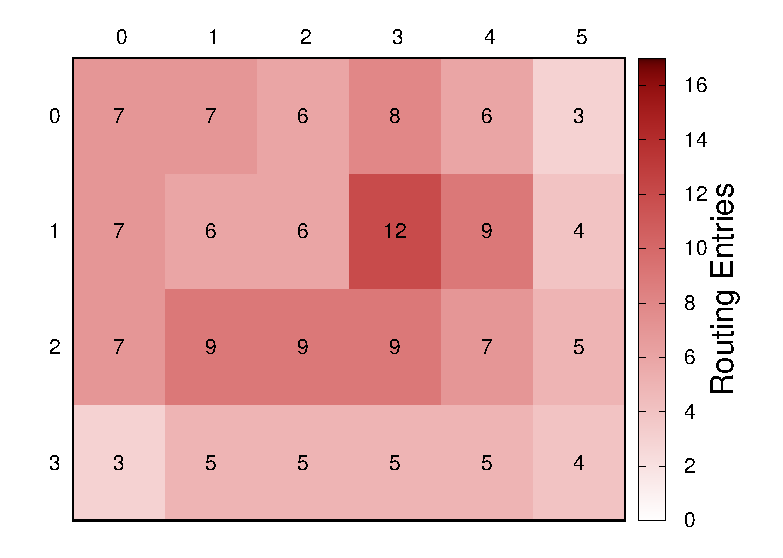
\includegraphics[width=1.0\linewidth]{charts/synth1/synth1-routing-tables-heatmap-sla-off-optimal.eps}
			\end{subfigure}
			\begin{subfigure}{0.45\linewidth}
				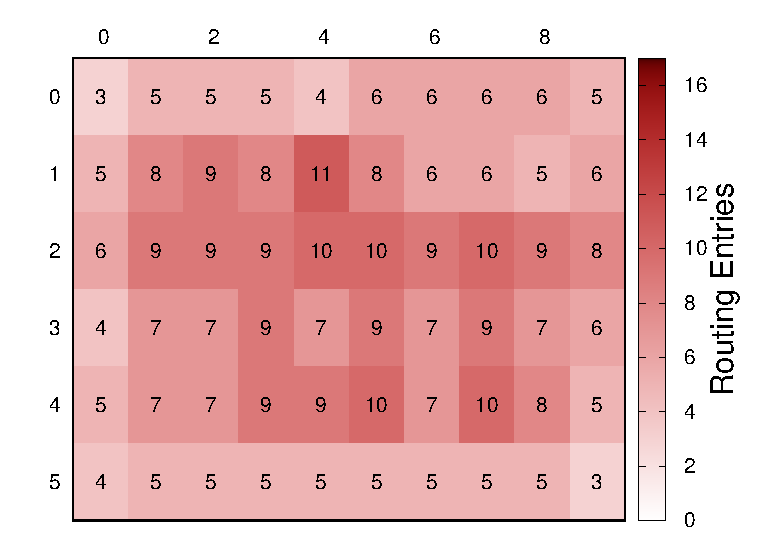
\includegraphics[width=1.0\linewidth]{charts/synth2/synth2-routing-tables-heatmap-sla-off-optimal.eps}
			\end{subfigure}
			\begin{subfigure}{0.45\linewidth}
				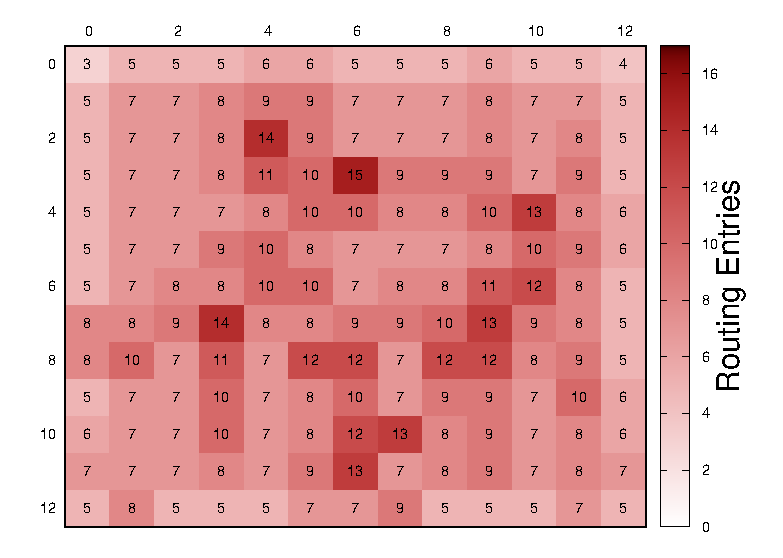
\includegraphics[width=1.0\linewidth]{charts/nasa/nasa-routing-tables-heatmap-sla-off-optimal.eps}
			\end{subfigure}
		\end{figure}
	\end{center}
\end{frame}

\begin{frame}{FIZ Occurrences}
	\begin{center}
		\begin{figure}
			\begin{subfigure}{0.49\linewidth}
				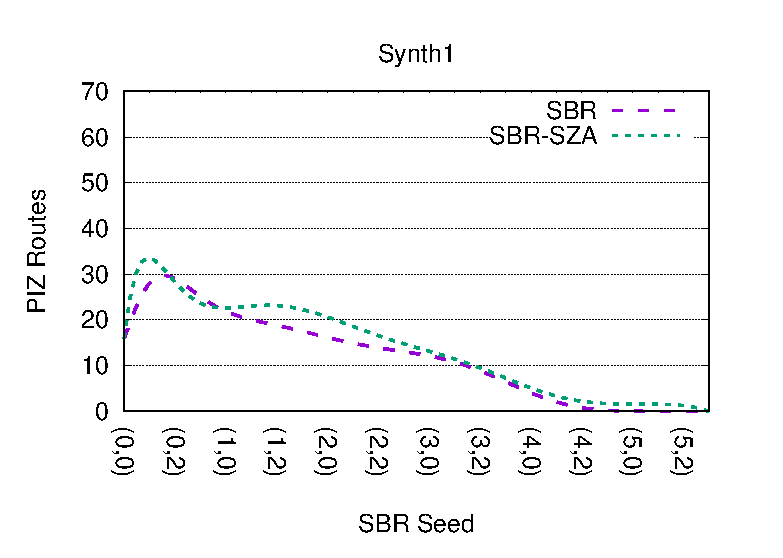
\includegraphics[width=1.0\linewidth]{charts/synth1/synth1-piz-routes-bezier.eps}
			\end{subfigure}
			\begin{subfigure}{0.49\linewidth}
				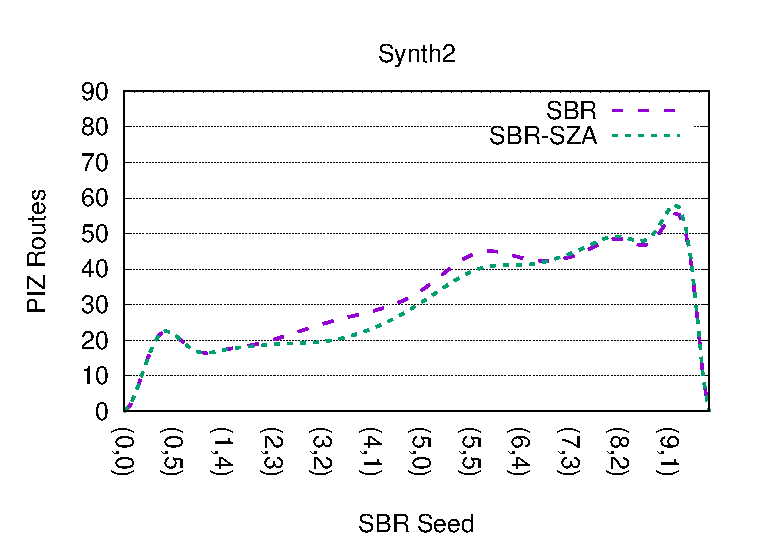
\includegraphics[width=1.0\linewidth]{charts/synth2/synth2-piz-routes-bezier.eps}
			\end{subfigure}
			\begin{subfigure}{0.49\linewidth}
				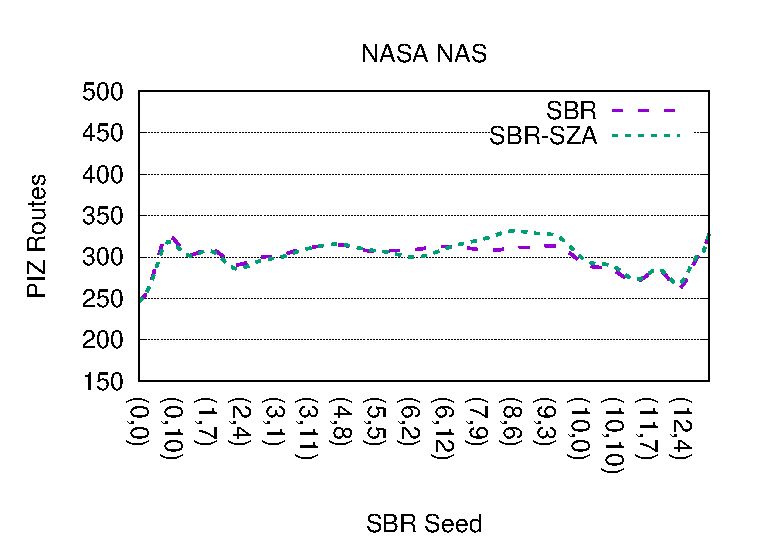
\includegraphics[width=1.0\linewidth]{charts/nasa/nasa-piz-routes-bezier.eps}
			\end{subfigure}
		\end{figure}
	\end{center}
\end{frame}

\begin{frame}{Latency Variation}
	\begin{center}
		\begin{figure}
			\begin{subfigure}{0.49\linewidth}
				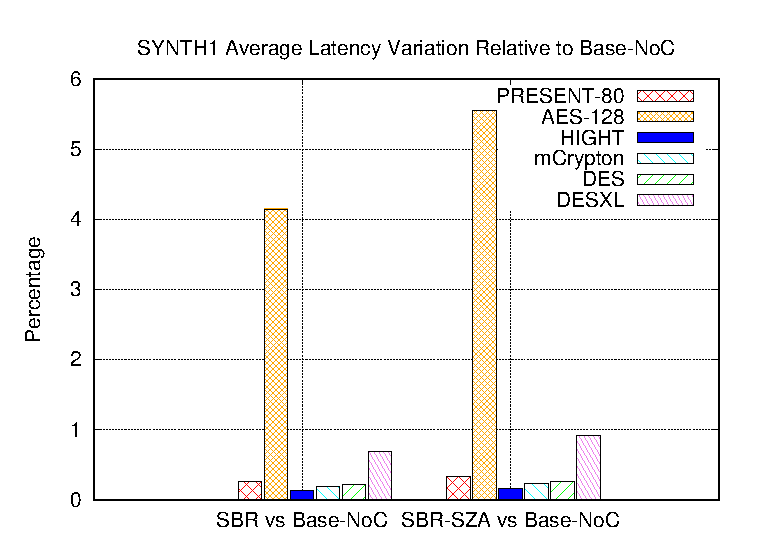
\includegraphics[width=1.0\linewidth]{charts/synth1/synth1-path-cost-comparison-relative.eps}
			\end{subfigure}
			\begin{subfigure}{0.49\linewidth}
				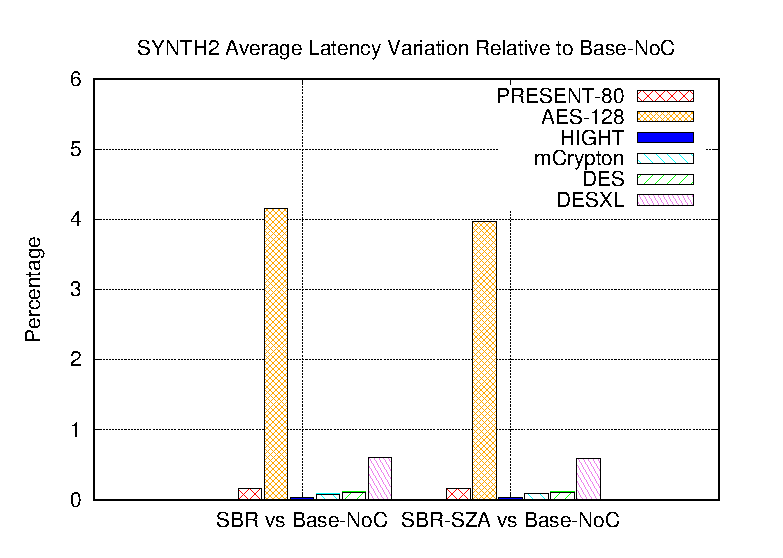
\includegraphics[width=1.0\linewidth]{charts/synth2/synth2-path-cost-comparison-relative.eps}
			\end{subfigure}
			\begin{subfigure}{0.49\linewidth}
				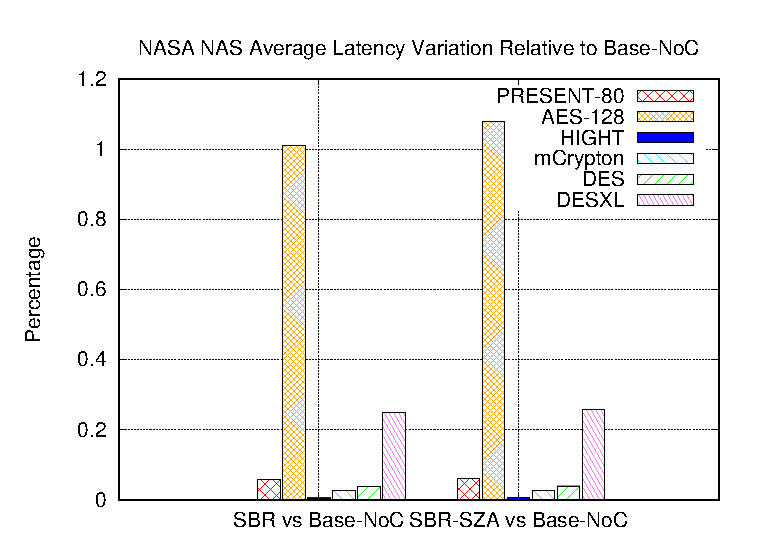
\includegraphics[width=1.0\linewidth]{charts/nasa/nasa-path-cost-comparison-relative.eps}
			\end{subfigure}
		\end{figure}
	\end{center}
\end{frame}

\begin{frame}{Latency Variation - FIZ Communication}
	\begin{center}
		\begin{figure}
			\begin{subfigure}{0.49\linewidth}
				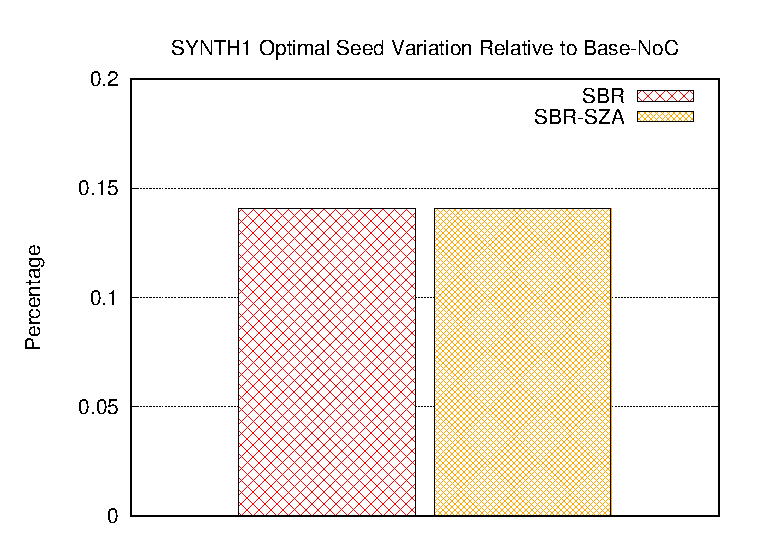
\includegraphics[width=1.0\linewidth]{charts/synth1/synth1-path-cost-comparison-optimal.eps}
			\end{subfigure}
			\begin{subfigure}{0.49\linewidth}
				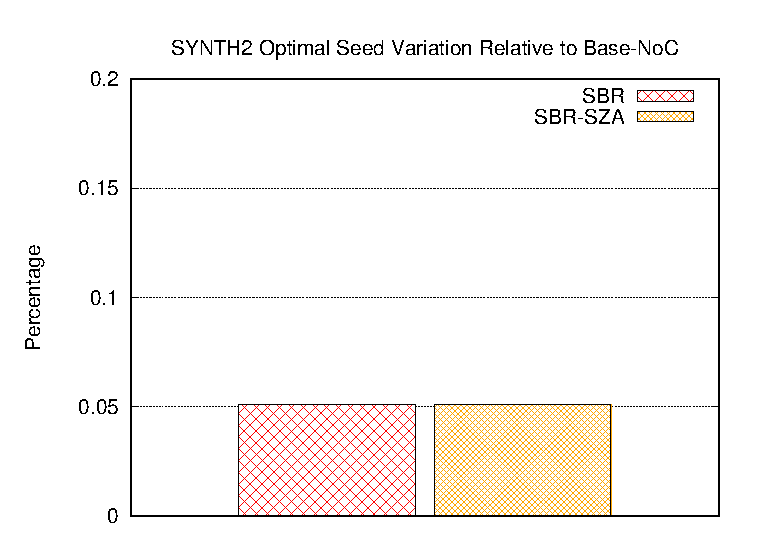
\includegraphics[width=1.0\linewidth]{charts/synth2/synth2-path-cost-comparison-optimal.eps}
			\end{subfigure}
		\end{figure}
	\end{center}
\end{frame}
	
	%%%%%%%%%%%%%%%%%%%%%%%%%%%%%%%%%%%%%%%%%%
	%%% WORK SCHEDULE %%%%%%%%%%%%%%%%%%%%%%%%
	%%%%%%%%%%%%%%%%%%%%%%%%%%%%%%%%%%%%%%%%%%
	\section{Work Schedule}\label{sec:work-schedule}
\begin{frame}{Work Schedule}
	\centering
	\resizebox{0.85\textwidth}{!}{
		\tabulinesep = 3pt
		\begin{tabu}{|X[16,c]|*{9}{X[1,c]|}}
			\cline{1-10}
			
			\multirow{2}{*}{Activities} & \multicolumn{6}{c|}{2016} & \multicolumn{3}{c|}{2017}
			
			\\ \cline{2-10}
			
			& 07 & 08 & 09 & 10 & 11 & 12 & 01 & 02 & 03
			
			\\ \cline{1-10}\hline
			
			Study of Related Work & \cellcolor{blue!50} & \cellcolor{blue!50} & \cellcolor{blue!50} & \cellcolor{blue!50} & \cellcolor{blue!50} & \cellcolor{blue!50} & \cellcolor{blue!50} & \cellcolor{blue!50} &
			
			\\ \cline{1-10}\hline
			
			SA Writing & \cellcolor{blue!50} & & & & & & & &
			
			\\ \cline{1-10}\hline
			
			SA Presentation & \cellcolor{blue!50} & & & & & & & &
			
			\\ \cline{1-10}\hline
			
			Dissertation Writing & & & & \cellcolor{blue!50} & \cellcolor{blue!50} & \cellcolor{blue!50} & \cellcolor{blue!50} & &
			
			\\ \cline{1-10}\hline
			
			Paper submission and writing & \cellcolor{blue!50} & \cellcolor{blue!50} & \cellcolor{blue!50} & \cellcolor{blue!50} & \cellcolor{blue!50} & \cellcolor{blue!50} & \cellcolor{blue!50} & \cellcolor{blue!50} &
			
			\\ \cline{1-10}\hline
			
			Creation of Configuration Scenarios and Traffic Generators & \cellcolor{blue!50} & \cellcolor{blue!50} & \cellcolor{blue!50} & \cellcolor{blue!50} & \cellcolor{blue!50} & \cellcolor{blue!50} & & &
			
			\\ \cline{1-10}\hline
			
			Model Evaluation and Result Analysis & \cellcolor{blue!50} & \cellcolor{blue!50} & \cellcolor{blue!50} & \cellcolor{blue!50} & \cellcolor{blue!50} & \cellcolor{blue!50} & & &
			
			\\ \cline{1-10}\hline
			
			Master's Degree Defense & & & & & & & & & \cellcolor{blue!50}
			
			\\ \cline{1-10}\hline
		\end{tabu}
	}
\end{frame}
	
	%%%%%%%%%%%%%%%%%%%%%%%%%%%%%%%%%%%%%%%%%%
	%%% QUESTIONS %%%%%%%%%%%%%%%%%%%%%%%%%%%%
	%%%%%%%%%%%%%%%%%%%%%%%%%%%%%%%%%%%%%%%%%%
	\begin{frame}
		\begin{center}
			{
				\huge
				Questions?	
			}
		\end{center}
	\end{frame}
	
	%%%%%%%%%%%%%%%%%%%%%%%%%%%%%%%%%%%%%%%%%%
	%%% BIBLIOGRAPHY %%%%%%%%%%%%%%%%%%%%%%%%%
	%%%%%%%%%%%%%%%%%%%%%%%%%%%%%%%%%%%%%%%%%%
%	\begin{frame}[allowframebreaks]
%		\printbibliography
%	\end{frame}
\end{document}